%% abtex2-modelo-artigo.tex, v-1.9.7 laurocesar
%% Copyright 2012-2018 by abnTeX2 group at http://www.abntex.net.br/
%%
%% This work may be distributed and/or modified under the
%% conditions of the LaTeX Project Public License, either version 1.3
%% of this license or (at your option) any later version.
%% The latest version of this license is in
%%   http://www.latex-project.org/lppl.txt
%% and version 1.3 or later is part of all distributions of LaTeX
%% version 2005/12/01 or later.
%%
%% This work has the LPPL maintenance status `maintained'.
%%
%% The Current Maintainer of this work is the abnTeX2 team, led
%% by Lauro César Araujo. Further information are available on
%% http://www.abntex.net.br/
%%
%% This work consists of the files abntex2-modelo-artigo.tex and
%% abntex2-modelo-references.bib
%%

% -----
% Versão adaptada para ENCITA
% Autoria Filipe Verri <verri@ita.br>
% Data 22/12/2021
% -----

% ------------------------------------------------------------------------
% ------------------------------------------------------------------------
% abnTeX2: Modelo de Artigo Acadêmico em conformidade com
% ABNT NBR 6022:2018: Informação e documentação - Artigo em publicação
% periódica científica - Apresentação
% ------------------------------------------------------------------------
% ------------------------------------------------------------------------

\documentclass[
	% -- opções da classe memoir --
	article,			% indica que é um artigo acadêmico
	10pt,				% tamanho da fonte
	oneside,			% para impressão apenas no recto. Oposto a twoside
	a4paper,			% tamanho do papel.
  twocolumn,			% para coluna dupla
	english,			% idioma adicional para hifenização
	brazil,				% o último idioma é o principal do documento
	sumario=tradicional,
	]{abntex2}


% ---
% PACOTES
% ---

% ---
% Pacotes fundamentais
% ---
\usepackage{lmodern}			% Usa a fonte Latin Modern
\usepackage[T1]{fontenc}		% Selecao de codigos de fonte.
\usepackage[utf8]{inputenc}		% Codificacao do documento (conversão automática dos acentos)
\usepackage{indentfirst}		% Indenta o primeiro parágrafo de cada seção.
\usepackage{nomencl} 			% Lista de simbolos
\usepackage{color}				% Controle das cores
\usepackage{graphicx}			% Inclusão de gráficos
\usepackage{microtype} 			% para melhorias de justificação
\usepackage{booktabs} % Tabelas
% ---

% ---
% Pacotes de citações
% ---
\usepackage[alf]{abntex2cite}	% Citações padrão ABNT
% ---

% --- Informações de dados para CAPA e FOLHA DE ROSTO ---
\titulo{Caracterização de sistema de propulsão a gás frio com vetorização de empuxo}
\ifthenelse{\equal{\ABNTEXisarticle}{true}}{%
\renewcommand{\maketitlehookb}{}
}{}

\autor{Pedro Kuntz Puglia\thanks{Instituto Tecnológico de Aeronáutica, pesquisador voluntário,
  \href{mailto:pepuglia@gmail.com}{pepuglia@gmail.com}.},
  Leonardo Gouvêa\thanks{Instituto Tecnológico de Aeronáutica, orientador}, Maurício Morales\thanks{Instituto Tecnológico de Aeronáutica, co-orientador}}

\local{Instituto Tecnológico de Aeronáutica, São José dos Campos, SP, Brasil}
\data{XXVII Encontro de Iniciação Científica do ITA -- XXVII ENCITA/2022}
% ---

% ---
% Configurações de aparência do PDF final

% alterando o aspecto da cor azul
\definecolor{blue}{RGB}{41,5,195}

% informações do PDF
\makeatletter
\hypersetup{%pagebackref=true,
		pdftitle={\@title},
		pdfauthor={\@author},
		colorlinks=true,       		% false: boxed links; true: colored links
    	linkcolor=blue,          	% color of internal links
    	citecolor=blue,        		% color of links to bibliography
    	filecolor=magenta,      		% color of file links
		urlcolor=blue,
		bookmarksdepth=4
}
\makeatother
% ---

% ---
% compila o indice
% ---
\makeindex
% ---

% ---
% Altera as margens padrões
% ---
\setlrmarginsandblock{2cm}{2cm}{*}
\setulmarginsandblock{1.5cm}{2.5cm}{*}
\checkandfixthelayout
% ---

% ---
% Espaçamentos entre linhas e parágrafos
% ---

% O tamanho do parágrafo é dado por:
\setlength{\parindent}{0.7cm}

% Controle do espaçamento entre um parágrafo e outro:
\setlength{\parskip}{0.1cm}

% Espaçamento simples
\SingleSpacing

% Espaçamento após título das Referências
\setlength\afterchapskip{\lineskip}

% ----
% Início do documento
% ----
\begin{document}

% Seleciona o idioma do documento (conforme pacotes do babel)
\selectlanguage{brazil}

% Retira espaço extra obsoleto entre as frases.
\frenchspacing

% ----------------------------------------------------------
% ELEMENTOS PRÉ-TEXTUAIS
% ----------------------------------------------------------

% página de titulo principal (obrigatório)
\maketitle

% resumo em português
\begin{resumoumacoluna}
Este trabalho apresenta o processo de desenvolvimento e caracterização de um sistema de vetorização de empuxo com motor a gás frio. O motor tem como requisito empuxo de \(2\;\mathrm{N}\) e \(5\;\mathrm{bar}\) de pressão de câmara. O método de vetorização escolhido para teste foi o de \textit{jet vane}. O motor construído apresentou divergências pequenas com os requisitos, tendo um impulso específico de \(46,6\;\mathrm{s}\). Este motor foi montado em um mecanismo de controle da lâmina defletora e esta montagem foi acoplada a uma balança de três componentes para caracterização das forças e momentos gerados. Como resultado final, obtiveram-se as derivadas de controle de força lateral e momento. Por fim, apresentaram-se os problemas metodológicos encontrados e \textit{trade-offs} de engenharia identificados para o sistema.
 \vspace{\onelineskip}

 \noindent
 \textbf{Palavras-chave}: propulsão, gás frio, vetorização de empuxo, controle.
\end{resumoumacoluna}
% ---

% ----------------------------------------------------------
% ELEMENTOS TEXTUAIS
% ----------------------------------------------------------
\textual
% ----------------------------------------------------------
% Introdução
% ----------------------------------------------------------
\section{Introdução}

A tecnologia de controle de vetorização de empuxo (ou TVC, do inglês \textit{thrust vector control}) é fundamental para a estabilidade e para o seguimento de trajetória dos foguetes, pois utiliza o direcionamento do empuxo do motor para controlar o veículo. Este trabalho busca iniciar uma linha de pesquisa brasileira sobre o assunto.

O desenvolvimento de sistemas propulsivos é baseado em coeficientes semi-empíricos que relacionam o empuxo propulsivo \(F\), a vazão mássica \(\dot{m}\) e as áreas da seção transversal da garganta \(A_t\) e da tubeira \(A_e\). O coeficientes de empuxo \(C_F\) e a velocidade característica \(C^*\) podem ser usados para calcular a vazão mássica do motor foguete com~\cite{Sutton}
\begin{equation}
  \label{eq:mass_flow}
  \dot{m} = \frac{F}{C^* C_F}
\end{equation}
ao passo que as áreas das seções transversais da garganta e da tubeira podem ser relacionadas pela razão de expansão \(\varepsilon\), dada por
\begin{equation}
  \varepsilon = \frac{A_e}{A_t}\label{eq:exp_ratio}
\end{equation} 

\textit{Jet vanes}, ou lâminas defletoras, consistem em placas imersas no escoamento supersônico à jusante da tubeira do motor foguete. Para pequenas deflexões, escoamento uniforme e espessura infinitesimal, é possível afirmar que a força lateral produzida pelo sistema é proporcional ao ângulo de deflexão~\cite{anderson}. 

A formulação mais usual de controle linear invariante no tempo define uma matriz de controle~\cite{fbsys}, cujas entradas são derivadas de controle, como por exemplo a derivada da força lateral em relação à deflexão da lâmina defletora \(\delta \), dada por
\begin{equation}
  F_{x\delta} = \frac{\mathrm{d} F_x}{\mathrm{d} \delta}\label{eq:control_derivative}
\end{equation}

Sendo assim, este trabalho tem por objetivo final caracterizar as derivadas de controle de um sistema de vetorização de empuxo com um motor foguete de gás frio de pequena escala (\(2\;\mathrm{N}\)), bem como caracterizar seus coeficientes propulsivos e \textit{trade-offs} de engenharia relacionado ao sistema de vetorização de empuxo.

\section{Materiais e métodos}

O sistema propulsivo foi projetado de maneira programática com o auxílio do CEA NASA~\cite{ceanasa} e sua interface programática RocketCEA~\cite{rocketcea}. Foram levantados como requisitos empuxo \(F = 2\;\mathrm{N}\), pressão de câmara \(p_c = 500\;\mathrm{kPa}\), temperatura do propelente \(T_{\mathrm{prop}} = 298,15\;\mathrm{K}\). Estes dados foram inseridos no código desenvolvido para cálculo das áreas das seções transversais de garganta e tubeira. A área da seção transversal da câmara foi escolhida empiricamente.

O motor a gás frio e o sistema de vetorização foram manufaturados em ABS por impressão 3D. Para as medidas de força em função da deflexão da lâmina, foi utilizada a balança de três componentes Plint \& Partners disponível no Laboratório de Engenharia Aeronáutica. Esta balança é capaz de medir \(F_x\), uma força horizontal, \(F_y\), uma força vertical, e \(M\), um momento, através da leitura de três extensômetros visíveis na Fig.~\ref{fig:diag_three_axis_scale}.

\begin{figure}[htbp]
  \centering
  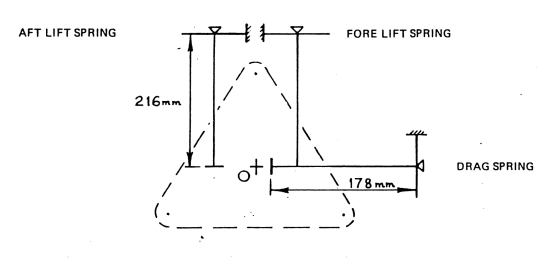
\includegraphics[width=\linewidth]{../report/img/three_axis_scale_diagram.png}
  \caption{Diagrama da balança de três componentes.}
  \label{fig:diag_three_axis_scale}
\end{figure}

A saída da balança, as forças \(F_A\) (\textit{aft}), \(F_F\) (\textit{fore}) e \(F_D\) (\textit{drag}) em cada extensômetro, podem ser convertidas nas forças horizontal, vertical e no momento atuante com o conhecimento da distância \(d\) entre as componentes \textit{aft} e \textit{fore}~\cite{lab}.

\section{Seções do artigo}

O corpo de texto segue a mesma formatação da introdução. Sugere-se que as seções sejam: 1.
Introdução; 2. Material e Métodos; 3. Resultados e Discussão; 4. Conclusões e
Recomendações; 5. Agradecimentos; por fim, Referências.

\subsection{Corpo do texto}

As equações matemáticas devem ser citadas como Eq. \ref{eq:mass-energy} no meio da
frase, ou por Equação \ref{eq:mass-energy} no início de uma frase.

Os símbolos usados nas equações devem ser definidos imediatamente antes ou depois de sua
primeira ocorrência no texto do trabalho: a equivalência massa-energia é dada por
\begin{equation}
  \label{eq:mass-energy}
  E = m c^2\mbox{,}
\end{equation}
onde $E$ é energia, $m$ a massa e $c$ a velocidade da luz no vácuo.

O tamanho da fonte usado nas equações deve ser compatível com o utilizado no texto. Todos
os símbolos devem ter suas unidades expressas no S.I. (Sistema Internacional).

As figuras devem ser centralizadas e referenciadas como Fig. \ref{fig:example} no meio da
frase ou por Figura \ref{fig:example}, caso apareçam no início. As anotações e numerações
devem ter tamanhos compatíveis com o da fonte usada no texto, e todas as unidades devem
ser expressas no S.I. (Sistema Internacional). Cada figura deve ser colocada na posição
mais próxima possível de sua primeira citação no texto. As legendas das figuras devem ser
alinhadas à esquerda.

\begin{figure}[h]
  \begin{center}
    \includegraphics[width=0.9\columnwidth]{example-image-a}
  \end{center}
  \caption{Exemplo de uma figura.}
  \label{fig:example}
\end{figure}

Figuras coloridas e fotografias de alta qualidade podem ser incluídas no trabalho. É
recomendável que qualquer figura inserida no trabalho tenha ao menos 90 DPI.

\begin{table*}[t]
  \caption{Resultados experimentais para as propriedades de flexão dos materiais MAT1 and
  MAT2. Valores médios de obtidos em 20 ensaios.}
  \label{tab:large}
  \centering
  \begin{tabular}{ccc}
    \toprule
    Propriedades do compósito & CFRC-TWILL & CFRC-4HS \\
    \midrule
    Resistência à Flexão (MPa) & $209\pm10$ & $180\pm15$ \\
    Módulo de Flexão (GPa) & $57\pm3$ & $18\pm1$ \\
    \bottomrule
  \end{tabular}
\end{table*}

As tabelas devem ser centralizadas e referidas por Tab. \ref{tab:example} no meio da
frase, ou por Tabela \ref{tab:example} no início de uma sentença. Os títulos das tabelas
devem ser localizados imediatamente acima da tabela. Anotações e valores numéricos nela
incluídos devem ter tamanhos compatíveis com o da fonte usada no texto do trabalho, e
todas as unidades devem ser expressas no S.I. (Sistema Internacional). As unidades são
incluídas apenas na primeira linha/coluna, conforme for apropriado. As tabelas devem ser
colocadas tão perto, o quanto possível, de sua primeira citação no texto. O estilo de
borda da tabela é livre. Exemplos são apresentados na Tab. \ref{tab:example} e na Tab.
\ref{tab:large}.

\begin{table}[h]
  \caption{Propriedades após o processamento.}
  \label{tab:example}
  \centering
  \begin{tabular}{ccc}
    \toprule
    Experimento & Prop. 1 (\%) & Prop. 2 (m)\\
    \midrule
    Ensaio 1 & $40.0$ & $22.7$ \\
    Ensaio 2 & $48.4$ & $13.9$ \\
    \bottomrule
  \end{tabular}
\end{table}

Referências aceitáveis incluem: artigos de periódicos, dissertações, teses, artigos
publicados em anais de congressos, ``preprints'', livros e artigos submetidos e aceitos em
revistas (identificar a fonte). Não citar páginas web, material didáticos, artigos em
blogs, vídeos ou similares.

\section{Agradecimentos}

Se bolsista, não esquecer de agradecimento à agência de fomento.

% ----------------------------------------------------------
% Referências bibliográficas
% ----------------------------------------------------------
\bibliography{artigo-encita}

\end{document}
